\PassOptionsToPackage{english, main = english}{babel}%% Suporte multilíngue

%% Classe e opções de documento
\documentclass[%% Opções
%%%% Opções da classe memoir
  article,%% Tipo de documento: article, book, report, etc.
  10pt,%% Tamanho de fonte: 10pt, 11pt, 12pt, etc.
  a4paper,%% Tamanho de papel: a4paper, letterpaper, etc.
  fleqn,%% Alinhamento de equações à esquerda (comente para centralizado)
  oneside,%% Impressão de elementos textuais e pós-textuais: oneside (anverso) ou twoside (anverso e verso)
  % twocolumn,%% Impressão em duas colunas (comente para uma coluna)
%%%% Opções da classe abntex2
  sumario = tradicional,%% Estilo de sumário: tradicional (padrão) ou abnt-6027-2012 (ABNT NBR 6027-2012)
  chapter = TITLE,%% Títulos de capítulos em maiúsculas (comente para desabilitar)
  section = TITLE,%% T\cite{ítulos de seções secundárias em maiúsculas (comente para desabilitar)
  % subsection = TITLE,%% Títulos de seções terciárias em maiúsculas (comente para desabilitar)
  % subsubsection = TITLE,%% Títulos de seções quartenárias em maiúsculas (comente para desabilitar)
]{abntex2}

%% Pacotes utilizados
\usepackage{report}%% Estilos do modelo
\usepackage{lipsum}%% Geração de texto fictício
\usepackage{algorithm}
\usepackage[noend]{algpseudocode}

%% Arquivo de referências
\addbibresource{report.bib}

%% Informações do documento
\titulo{%% Título
  Scientific Computing - Practice sessions%
}
\tituloemoutroidioma{%% Título em outro idioma
  Audio command recognition by DTW and classification%
}
\author{
  21906085\\
  Duc Thang, NGUYEN\\
  \texttt{duc-thang.nguyen@univ-tlse3.fr}
  \and
   21902771\\
  Clement, POULL\\
  \texttt{clement.poull@univ-tlse3.fr}
}

\instituicao{\utfprname}%% Instituição --- Automático
%\campus{PG}{}%% Câmpus: {sigla} e {nome}
\departamento[logo_FSI.jpg]{<DEPTO>}{%% Depto., Coord., Prog. ou Curso: [logo], {sigla} e {nome}
  Faculty of Science and Engineering%
}
%\local{Ponta Grossa, Paraná, Brasil}%% Local
%\data{}%% Data --- Comente para gerar a data atual

%% Ferramenta para criação de índices
\makeindex

%% Início do documento
\begin{document}

\pretextual%% Elementos pré-textuais

\begin{paginadetitulo}%% Página de título

\begin{ambienteresumo}[Abstract]%% Abstract
\begin{otherlanguage*}{english}%% Idioma do abstract
Speech recognition can be used in many fields, including command recognition for voice drone control. The state of the arts methods for spoken word recognition often base on MFCCs (Mel Frequency Cepstral Coefficients) to extract feature of audio. In this report, we present some approaches to classify the 13 drone commands in French. Firstly, We use dynamic time warping (DTW) algorithm. Second approach, using Principal Component Analysis (PCA) to get feature data reduction of MFCC and then apply k-nearest neighbors (KNN) to classify them. A upgrade of this approach, we combine MFCC and Delta Coefficients to get more features about sound and frame signals change. And finally, we use Convolution neural networks (CNN) into MFCCs directly. The dataset is composed of  235 records without noise and 53 records with noise from 13 native speakers. We use 80\% of our dataset to train model, 20\% dataset to test and measure the accuracy of approaches. During training, we augment data to variety of situations dataset like pitch, shift, stretch, ignore noise,\dots The best results base on F1 score, when we use DTW is 83\%, PCA + KNN is 91\% and CNN is 89\%. We also evaluate independently on own dataset (39 files) from native accent and Vietnamese accent with DTW is 79\%, PCA + KNN is 95\% and CNN is 79\%.

\smallskip

\textbf{Source code:} https://github.com/thangdnsf/Audio-command-recognition
\palavraschave[Keywords]{DTW, PCA, KNN, MFCC, delta coef, CNN, Speech Recognition}%% Keywords

\end{otherlanguage*}
\end{ambienteresumo}

\end{paginadetitulo}

\textual%% Elementos textuais

\section{Introduction}\label{sec:intro}

The pattern speech recognition is rapidly applying in may domains including, health care, military, and telephony,\dots Which can identify the pattern of content base on the form of wave that reflects physiologic and behavior characteristics from speaker that is called the feature extraction process. There are many feature extraction methods exist for audio but Mel Frequency Cepstral Coefficients (MFCCs) algorithm is a the state of the art method have been widely used. Then they used to classify or measure distance between datas. There are many the state of the art methods to do that such as: Dynamic time warping (DTW), KNN, Neural Network,\dots In this report, we will implement DTW algorithm, KNN and Convolution Neural networks.

%Then they are applied PCA to reduce the size of feature dimension and keep important features. Using PCA before training model such as:  KNN, SVM, Neural Networks, \dots will enable our classification model to seed up and more accuracy.

In our case, it will be used to give voice commands for controlling a drone. Unlike direct control methods such as a menu, speech recognition is not trivial and is not always flawless. The computer has no way to directly execute what the speech represents but needs to interpret the voice before execution. This can prove troublesome when the sample has noise, inconsistent speed, volume and many more parameters that can degrade their quality.

As a result, we need a way to accurately interpret the voice commands as one of 13 instructions for controlling a drone: \textit{arretetoi}, \textit{atterrissage}, \textit{avance}, \textit{decollage}, \textit{droite}, \textit{etatdurgence}, \textit{faisunflip}, \textit{gauche}, \textit{plusbas}, \textit{plushaut}, \textit{recule}, \textit{tournedroite}, \textit{tournegauche}.

In the next section will explain about methodology, results, and conclusions. In section II will be explained about the methodology of speech reconciliation process in detail. In the section III will be demonstrate the our results, while section IV show the conclusions. 
%The final goal is to recognize these isolated instructions given in our voice as accurately as possible and compare the results of the DTW algorithm with PCA preprocessing and KNN classification.

\section{Methodology}\label{sec:met}
In this section, we will present and explain more detail about the speech recognition process on each approaches.

First of all, we present briefly the dataset and take prepossessing data.
\subsection{Dataset and prepossessing}
The dataset we had access to was composed of sets of the 13 instructions spoken by 13 native speakers in different conditions with audio parameters: 16 KHz, mono, 16 bits, .wav format. The total of dataset include 235 records without noise (by 13 males and 5 females) and 53 records (by 4 males) .
%It can be divided into 2 categories: 4 sets where voices of males with a high level of noise, 13 sets where voices of males with no noise and 5 sets where voices of females with no noise. 
During record dataset, Speaker often silent before and after speak word. So the audio file usually has silent two sides of main wave as shown Figure \ref{fig:sample_1}. So we need to cut the silent parts of the sample as Figure \ref{fig:sample_2} using trim method in librosa library with threshold to consider as silence is 30.
%Each sample is isolated but not reduced to only the instruction, so we need to cut the empty parts of the sample, as shown by the two following figures.

\begin{figure}[H]
  \centering
  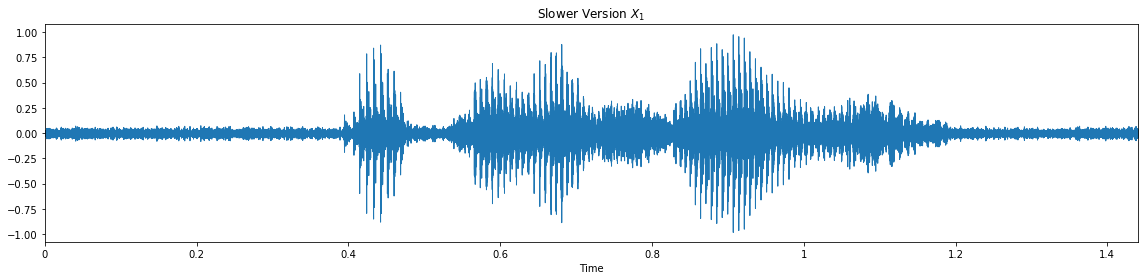
\includegraphics[width = 0.8\columnwidth]{./Figuras/sample_1}
   \caption{Sample before trimming.}
  \label{fig:sample_1}
\end{figure}

\begin{figure}[H]
  \centering
   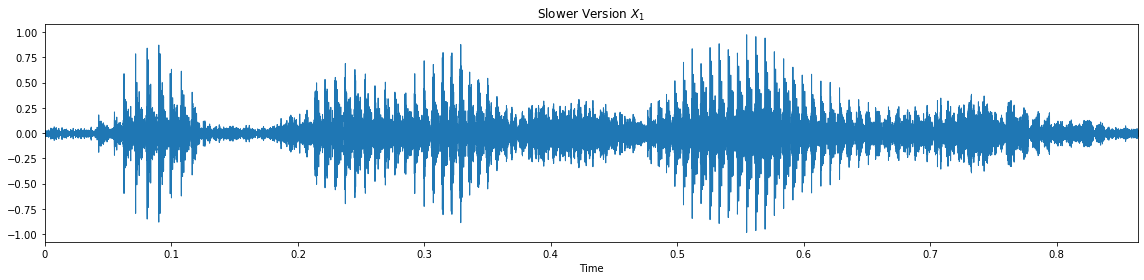
\includegraphics[width = 0.8\columnwidth]{./Figuras/sample_2}
    \caption{Sample after trimming.}
  \label{fig:sample_2}
\end{figure}

And the next task needs to reduce noise which affects the quality of audio and accuracy of the model by using noise reduction library based on algorithm by Audacity and get result as Figure \ref{fig:sample_3}.
\begin{figure}[H]
  \centering
   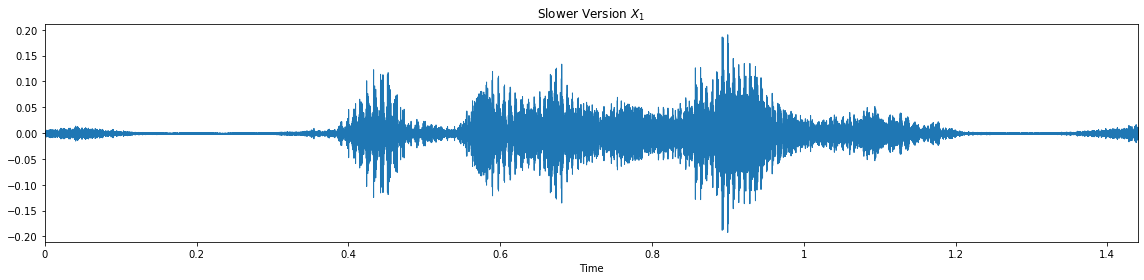
\includegraphics[width = 0.8\columnwidth]{./Figuras/sample_3}
    \caption{Sample after remove silent two sides.}
  \label{fig:sample_3}
\end{figure}

We use 80\% of our dataset to train model, 20\% dataset to test and measure the accuracy of approaches. During training, we has augmented data to variety of situations dataset like pitch, shift, stretch, ignore noise,\dots

\subsection{Feature extraction}

After data prepossessing, we will need to extract important features of each audio. One of the sate of the art methods is the mel-frequency cepstral coefficients (MFCCs) algorithm. MFCC is a frequency warping method that allows for a better representation of the response the human earring has, since it does not follow a linear scale. It calculates coefficients by performing a Fourier transform, mapping the result to the mel scale, taking the logs of the powers at certain frequencies, taking the discrete cosine transform of the logs and getting the amplitudes of the resulting spectrum. Figure \ref{fig:mfcc} is a sample of 'etadurgence' word. 

\begin{figure}[H]
  \centering
  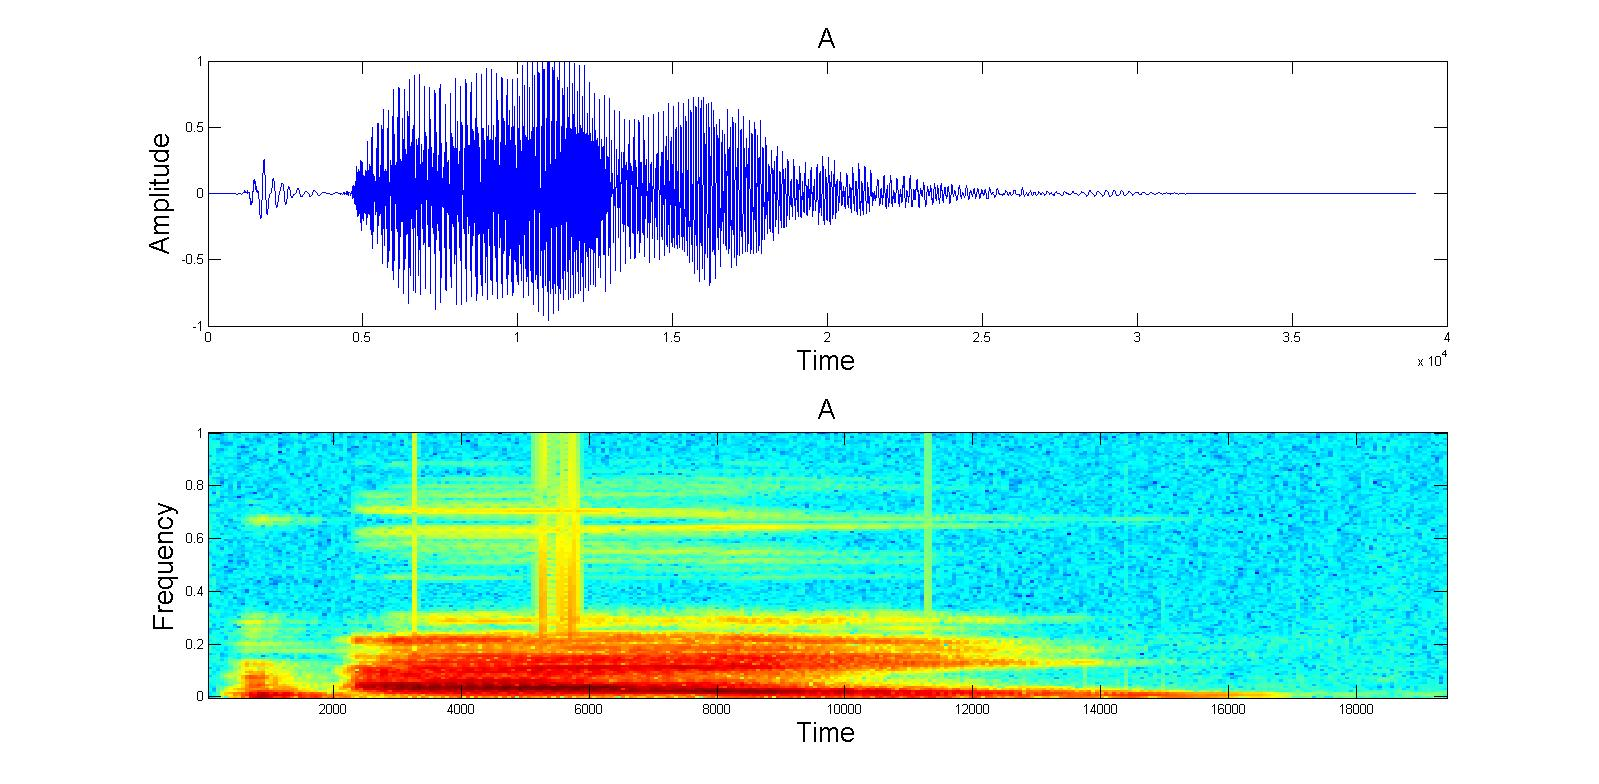
\includegraphics[width = 0.8\columnwidth]{./Figuras/mfcc}
  \caption{MFCC of 'etadurgence' word}
  \label{fig:mfcc}
 \end{figure}

To get more accuracy, we use Delta Coefficients and Delta Coefficients order 2 to extract feature regarding frame signals change, like the slope of a formant on the transition show example as figure \ref{fig:mfccdel}.
\begin{figure}[H]
  \centering
  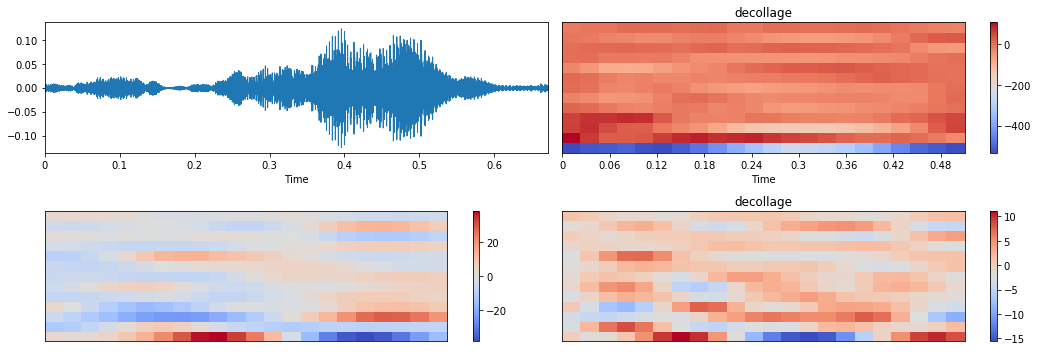
\includegraphics[width = 0.8\columnwidth]{./Figuras/mfcc_del}
  \caption{MFCC, del, del 2 of 'decollage' word}
  \label{fig:mfccdel}
 \end{figure}

\subsection{Methods}

\subsubsection{Dynamic time warping}
The Dynamic time warping (DTW) algorithm is showed in Algorithm\ref{euclid} is a popular method for comparing two sequences and illustrated by Figure \ref{fig:dtw_1}.

\begin{algorithm}
  \caption{DTW algorithm}\label{euclid}
  \begin{algorithmic}
    \State $g(0, 0) \gets 0$
    \For {$j \gets 1 \textit{ to } J$}
    \State $g(0, j) \gets +\infty$
    \EndFor
    \For {$i \gets 1 \textit{ to } I$}
    \State $g(i, 0) \gets +\infty$
    \For {$j \gets 1 \textit{ to } J$}
    \State $g(i, j) \gets min(g(i - 1, j) + \omega_{0} * d(i, j), g(i - 1, j - 1) + \omega_{1} * d(i, j), g(i, j - 1) + \omega_{2} * d(i, j))$
    \EndFor
    \EndFor
    \State $D \gets g(I, J) / (I + J)$
  \end{algorithmic}
\end{algorithm}
\begin{figure}[H]
  \centering
   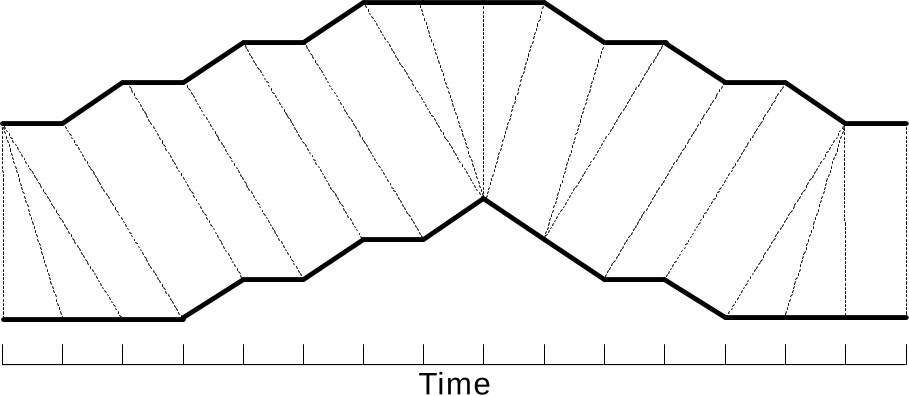
\includegraphics[width = 0.5\columnwidth]{./Figuras/dtw_1}
  \caption[Warping between two time series]{Warping between two time series\footnotemark.}
  \label{fig:dtw_1}
\end{figure}\footnotetext{Florida Institute of Technology}

And Figure \ref{fig:dtwmfcc} illustrates the comparison of two MFCCs using DTW \cite{1163055}.

\begin{figure*}
\centering
\begin{minipage}[b]{.3\textwidth}
\begin{figure}[H]
  \centering
  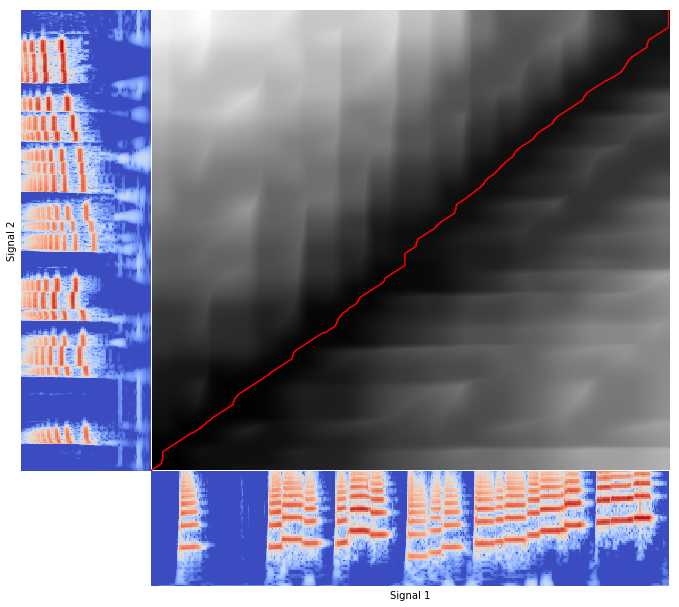
\includegraphics[width = \columnwidth]{./Figuras/dtwmfcc}
\end{figure}
\end{minipage}\qquad
\begin{minipage}[b]{.6\textwidth}
\begin{figure}[H]
  \centering
  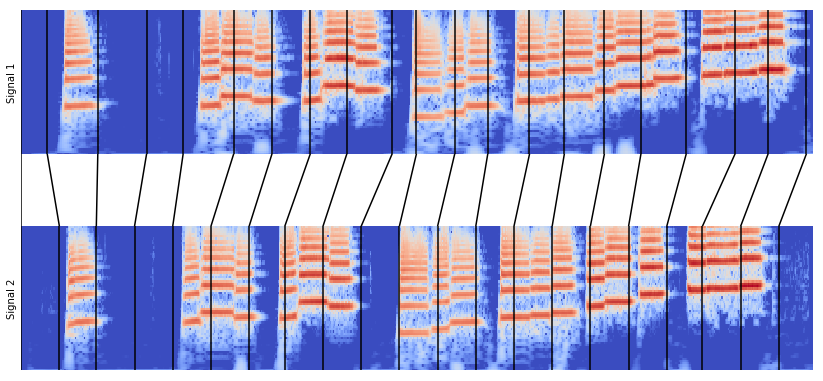
\includegraphics[width = \columnwidth]{./Figuras/mfccdtw2}
\end{figure}
\end{minipage}
\caption[css]{Compare two MFCCs using DTW\footnotemark}
\label{fig:dtwmfcc}
\end{figure*}
\footnotetext{musicinformationretrieval.com}

The first part our recognition method uses the dynamic time warping (DTW) algorithm on the MFCCs of each samples present in Algorithm \ref{mfccdtw}.

\begin{algorithm}
  \caption{MFCCs classification using DTW}\label{mfccdtw}
  \begin{algorithmic}
    \State $y\_pred = []$
    \For {$x \gets X\_test$}
    	\State $min\_dist \gets +\infty$
	\State $min\_index = None$
   	 \For {$x\_train,y\_train \gets X\_train, Y\_train$}
   		 \State $dist \gets dtw(x^T, x\_train^T)$
    		\If {$min\_dist > dist$}
    			\State $min\_dist \gets dist$
			\State $min_index = y\_train$
    		\EndIf
    	\EndFor
	\State $y\_pred \gets min_index$
    \EndFor
  \end{algorithmic}
\end{algorithm}

\subsection{PCA and KNN}
The second approach of our recognition method is to apply the principal component analysis (PCA) on our dataset, before classification with the KNN algorithm. PCA is a method that allows to reduce the size of a set by transforming it into a set of linearly uncorrelated variable. It works by calculating the co-variance matrix of the sequence, then by calculating the eigenvalues and eigenvectors of this matrix, choosing a subset of these eigenvectors and projecting the dataset onto a new basis created by the chosen eigenvectors\cite{8538414}. Note that, we need to fix size of all data by padding zeros vector to two slide of each MFCC Figure \ref{fig:mfccpadding} and flatten each MFCC to vector. and Then rescaling our data to a range between -1 and 1, with StandardScaler method from sklearn. 

\begin{figure}[H]
  \centering
  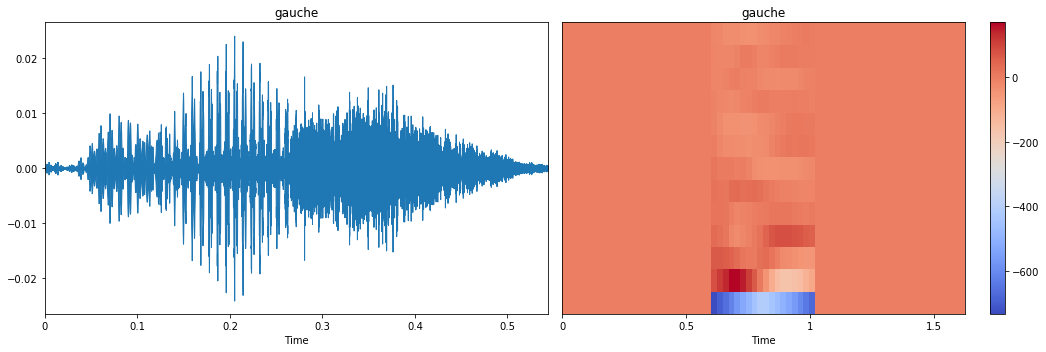
\includegraphics[width = 0.8\columnwidth]{./Figuras/mfccpadding}
  \caption{Fix size MFCC by padding zero vectors}
  \label{fig:mfccpadding}
\end{figure}

And the we will classify via classification algorithms like KNN, SVM, Neural networks, \dots  We will perform the K-nearest neighbors (KNN) using KNN method in sklearn library. It works by having a training base, on which is placed a test sample. The training base is composed of vectors with each an associated label, the label on these training vectors represents a class. We then check the neighborhood of the test sample, and take its k closest neighbors. These neighbors are then used to classify the test sample, with techniques such as majority voting, or weighted majority voting.

\begin{figure}[H]
  \centering
  \caption{KNN with two classes.}
  \label{fig:knn}
  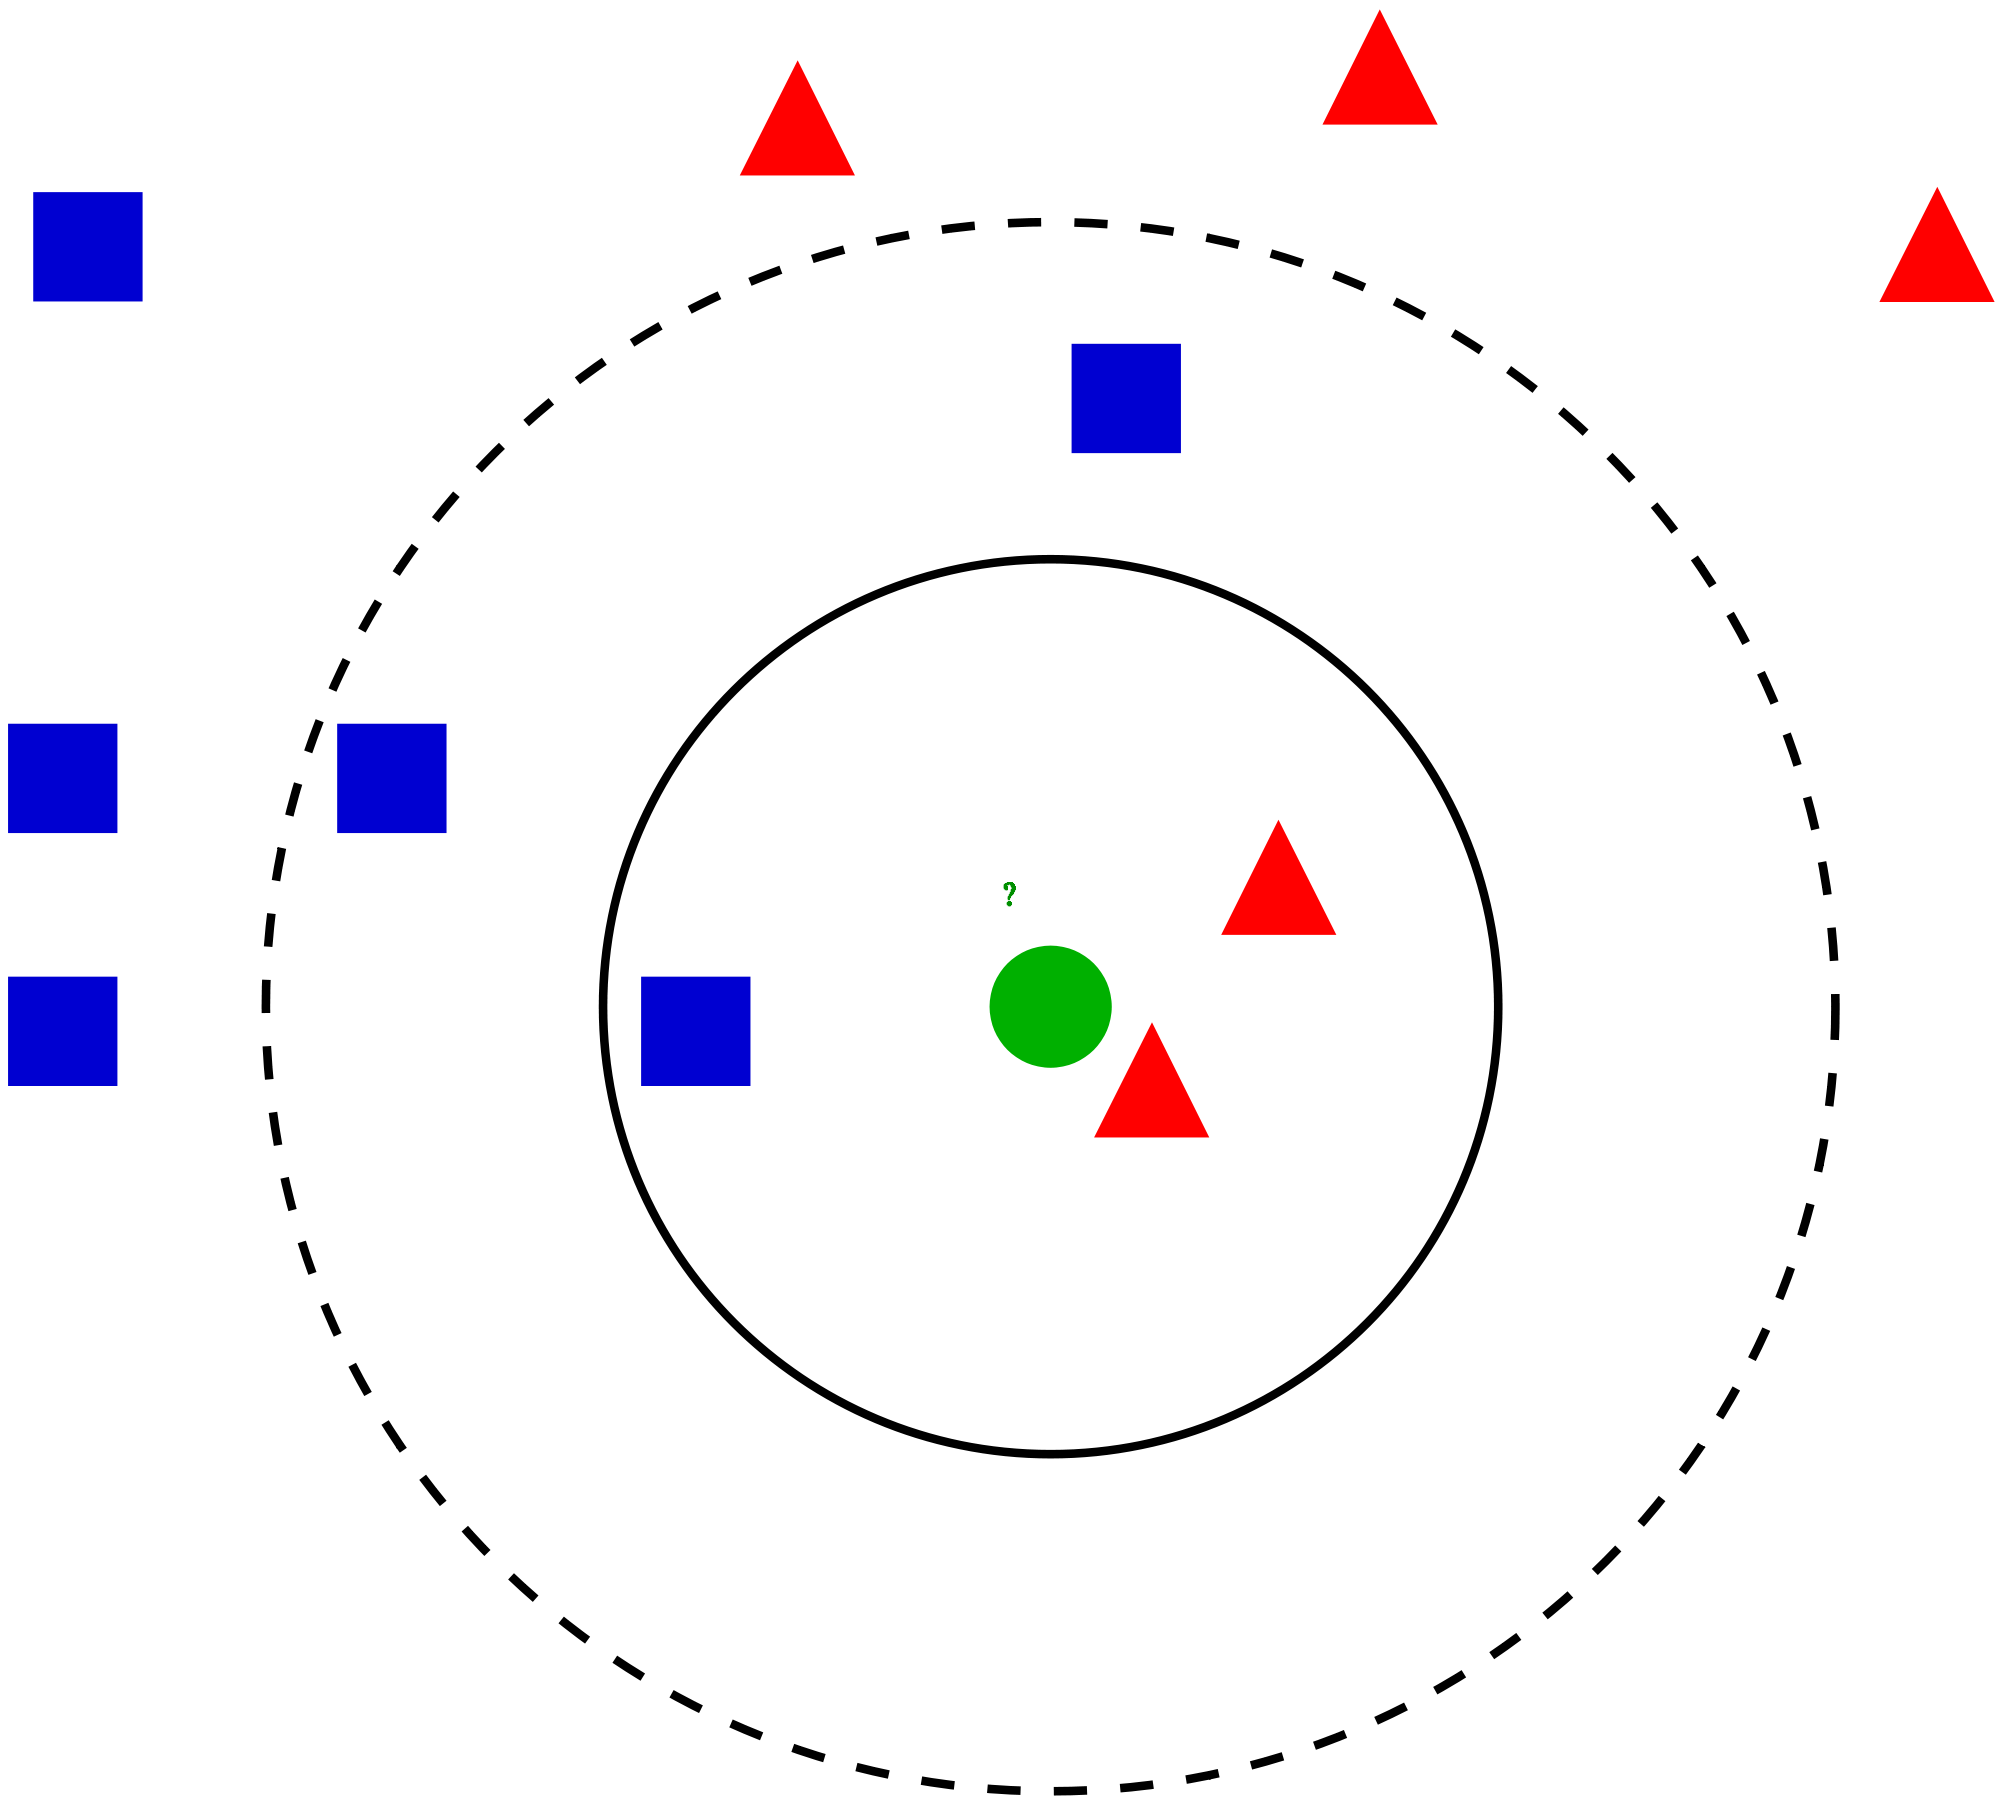
\includegraphics[width = 0.5\columnwidth]{./Figuras/knn}
\end{figure}

\subsection{Convolutions neural networks}
The convolutions neural networks (CNN) is a neural network that has one or many convolutional layers as Figure\ref{fig:cnn} and are used mainly for image processing, classification, segmentation, \dots And this problem, we apply CNN model with our dataset as a image dataset where a MFCC matrix as a image.

\begin{figure}[H]
  \centering
  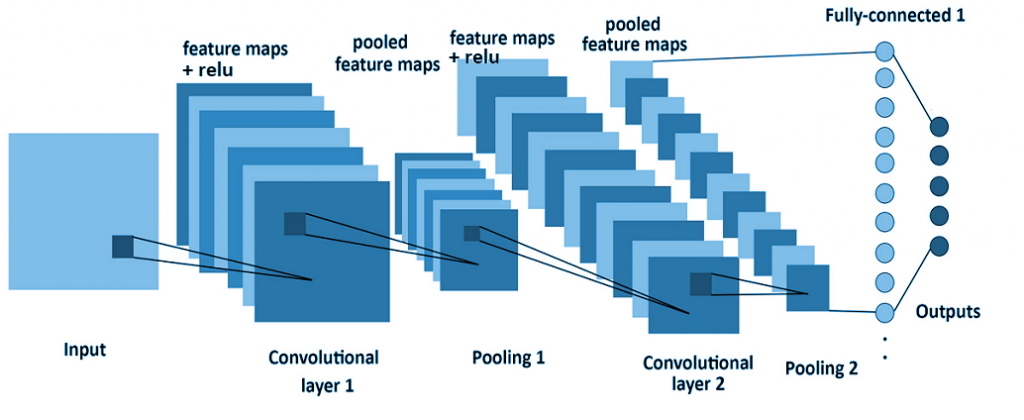
\includegraphics[width = 0.8\columnwidth]{./Figuras/cnn-1-1024x420}
  \caption{Convolutions neural networks.}
  \label{fig:cnn}
\end{figure}

\section{Performed tests and Results}\label{sec:res}
In this section, we will implement and present our above proposal methods in more detail. All our experiments are performed in python programming language and using jupyter notebook editor. To evaluate independently, we have recorded own dataset (39 files )by native and Vietnamese accent.

\subsection{DTW}
We have implemented Algorithm \ref{euclid} and evaluated by solving exercise TD2 as Figure \ref{fig:ex1} and \ref{fig:ex2}.

\begin{figure*}
\centering
\begin{minipage}[b]{.4\textwidth}
\begin{figure}[H]
  \centering
  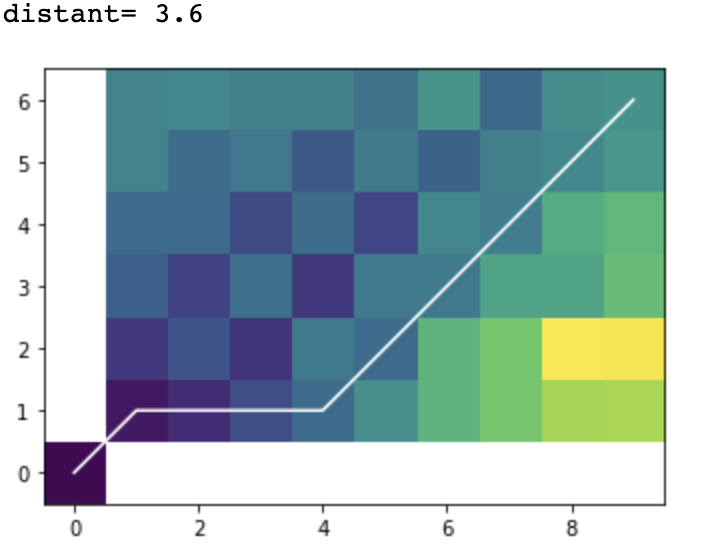
\includegraphics[width = \columnwidth]{./Figuras/ex1}
  \caption{Comparing two numerical sequences}
  \label{fig:ex1}
\end{figure}
\end{minipage}\qquad
\begin{minipage}[b]{.4\textwidth}
\begin{figure}[H]
  \centering
  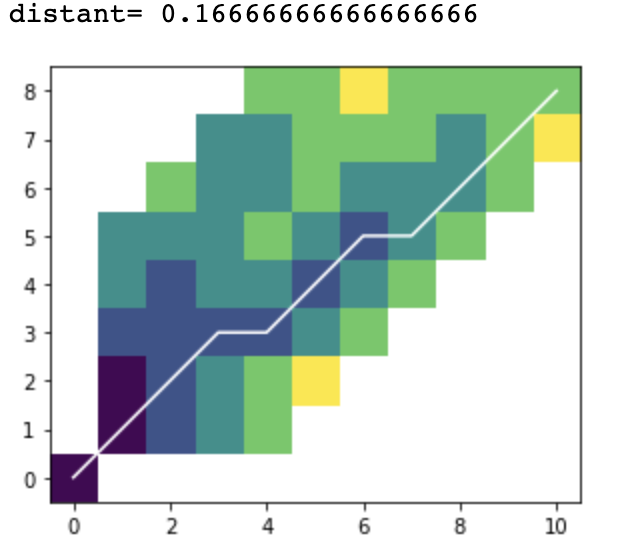
\includegraphics[width = \columnwidth]{./Figuras/ex2}
   \caption{Comparing DNA sequences}
   \label{fig:ex2}
\end{figure}
\end{minipage}
\end{figure*}

And then, we have evaluated performance of DTW algorithm with the following cases. Firstly, Evaluating influence male/ female voices and we have got so good result as Figure \ref{fig:dtwmalevsfemale}. Secondly, Evaluating influence background noises on recognition (learning set is data without noise and test set is data with noise) and we have got bad result as Figure \ref{fig:dtwnoiseonly}. Thirdly, Evaluating with normal (random noise and without noise) data as Figure \ref{fig:dtwall}. And finally, evaluating ability to new voice as Figure \ref{fig:dtwnewvoice}
\begin{figure*}
\centering
\begin{minipage}[b]{.4\textwidth}
\begin{figure}[H]
  \centering
  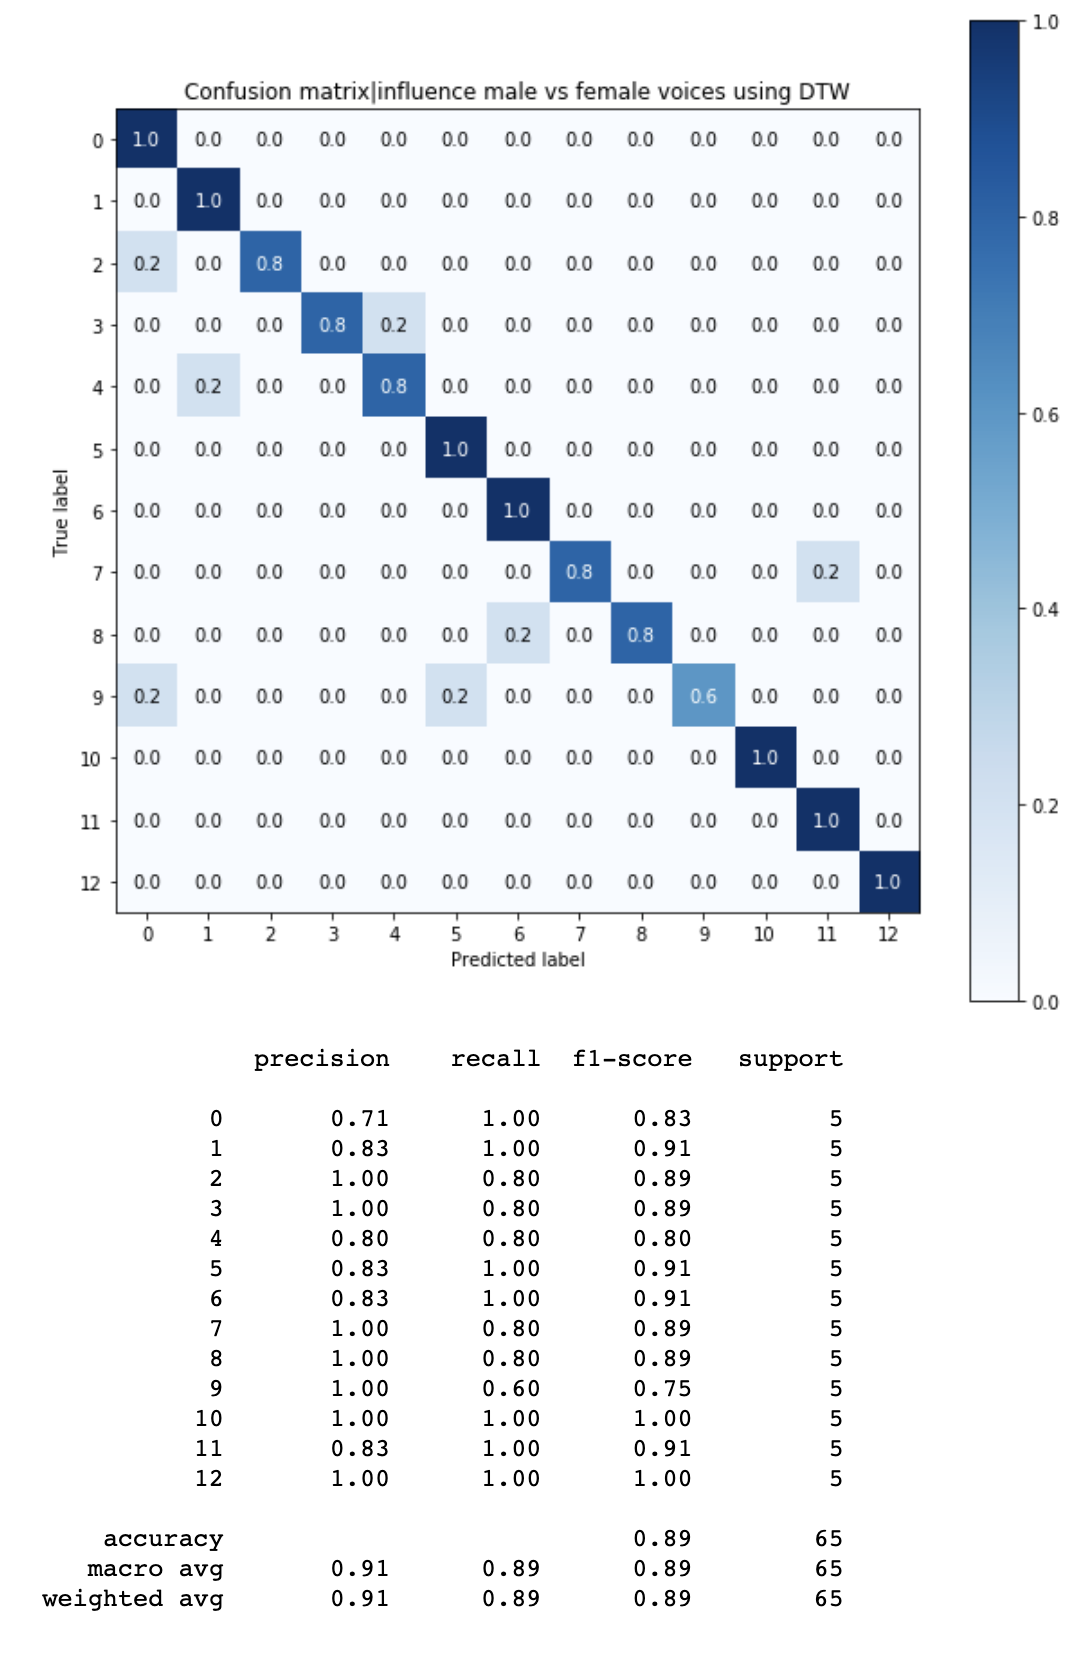
\includegraphics[width = \columnwidth]{./Figuras/dtwmalefemale}
  \caption{Evaluating DTW algorithm influence male/ female voices}
  \label{fig:dtwmalevsfemale}
\end{figure}
\end{minipage}\qquad
\begin{minipage}[b]{.4\textwidth}
\begin{figure}[H]
  \centering
  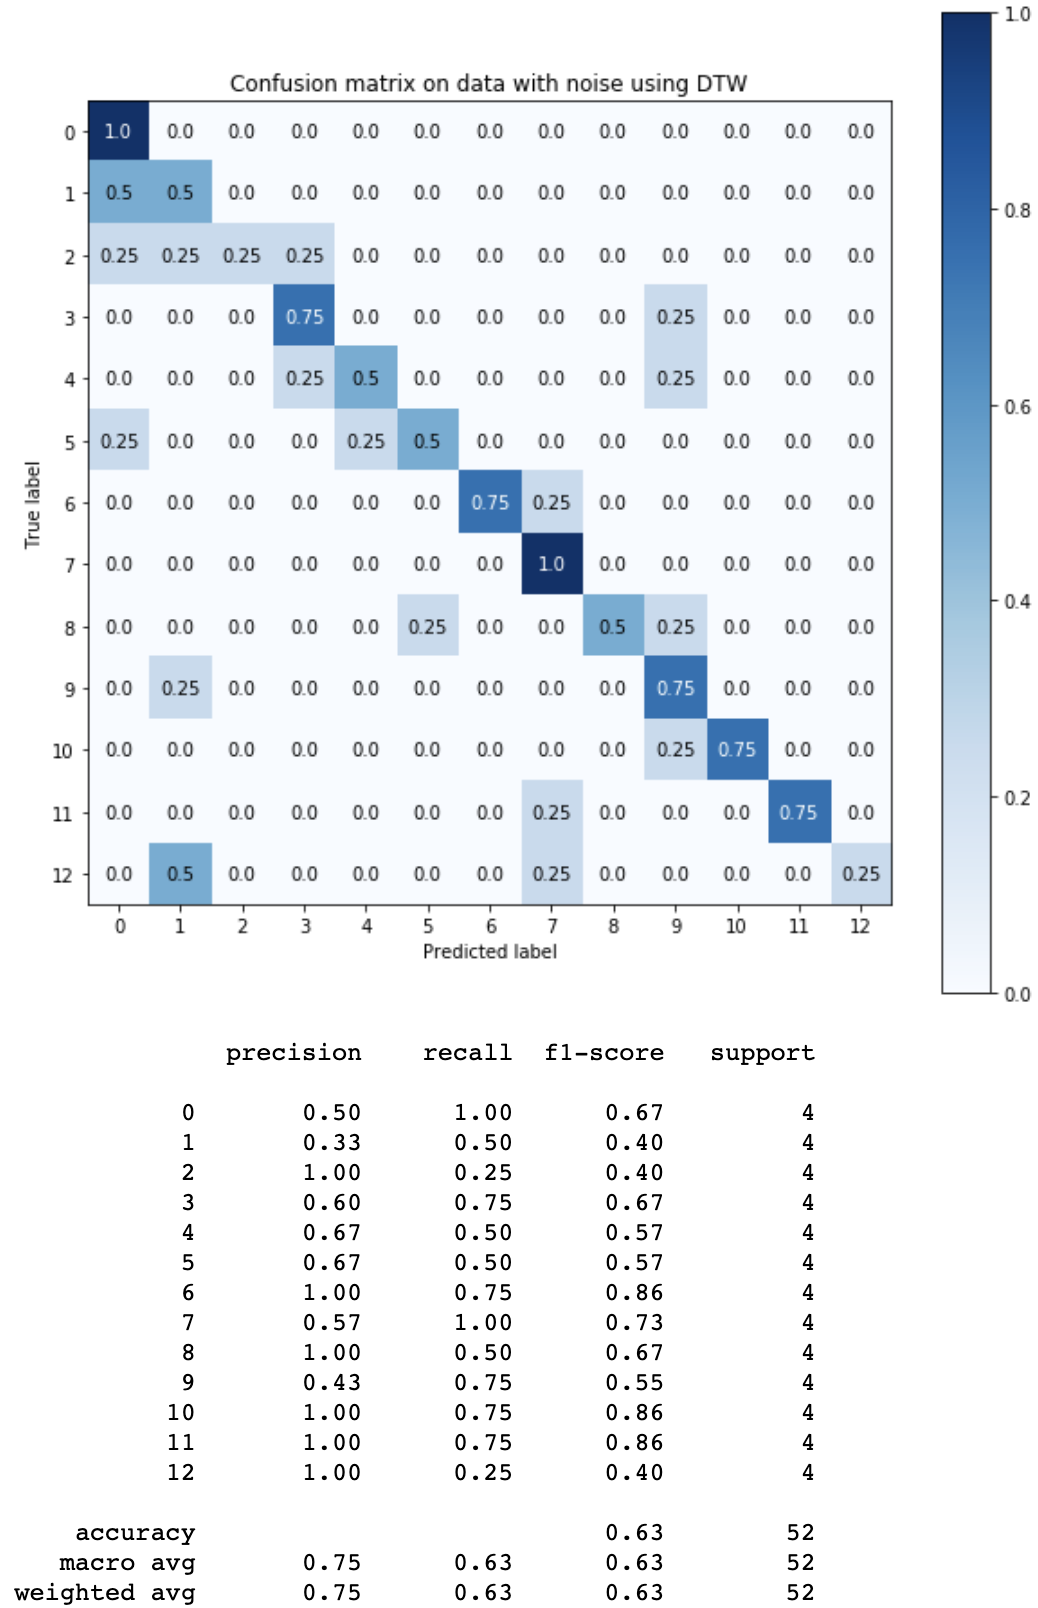
\includegraphics[width = \columnwidth]{./Figuras/dtwnoise}
   \caption{Evaluating DTW algorithm influence background noises on recognition}
   \label{fig:dtwnoiseonly}
\end{figure}
\end{minipage}
\end{figure*}

\begin{figure*}
\centering
\begin{minipage}[b]{.4\textwidth}
\begin{figure}[H]
  \centering
  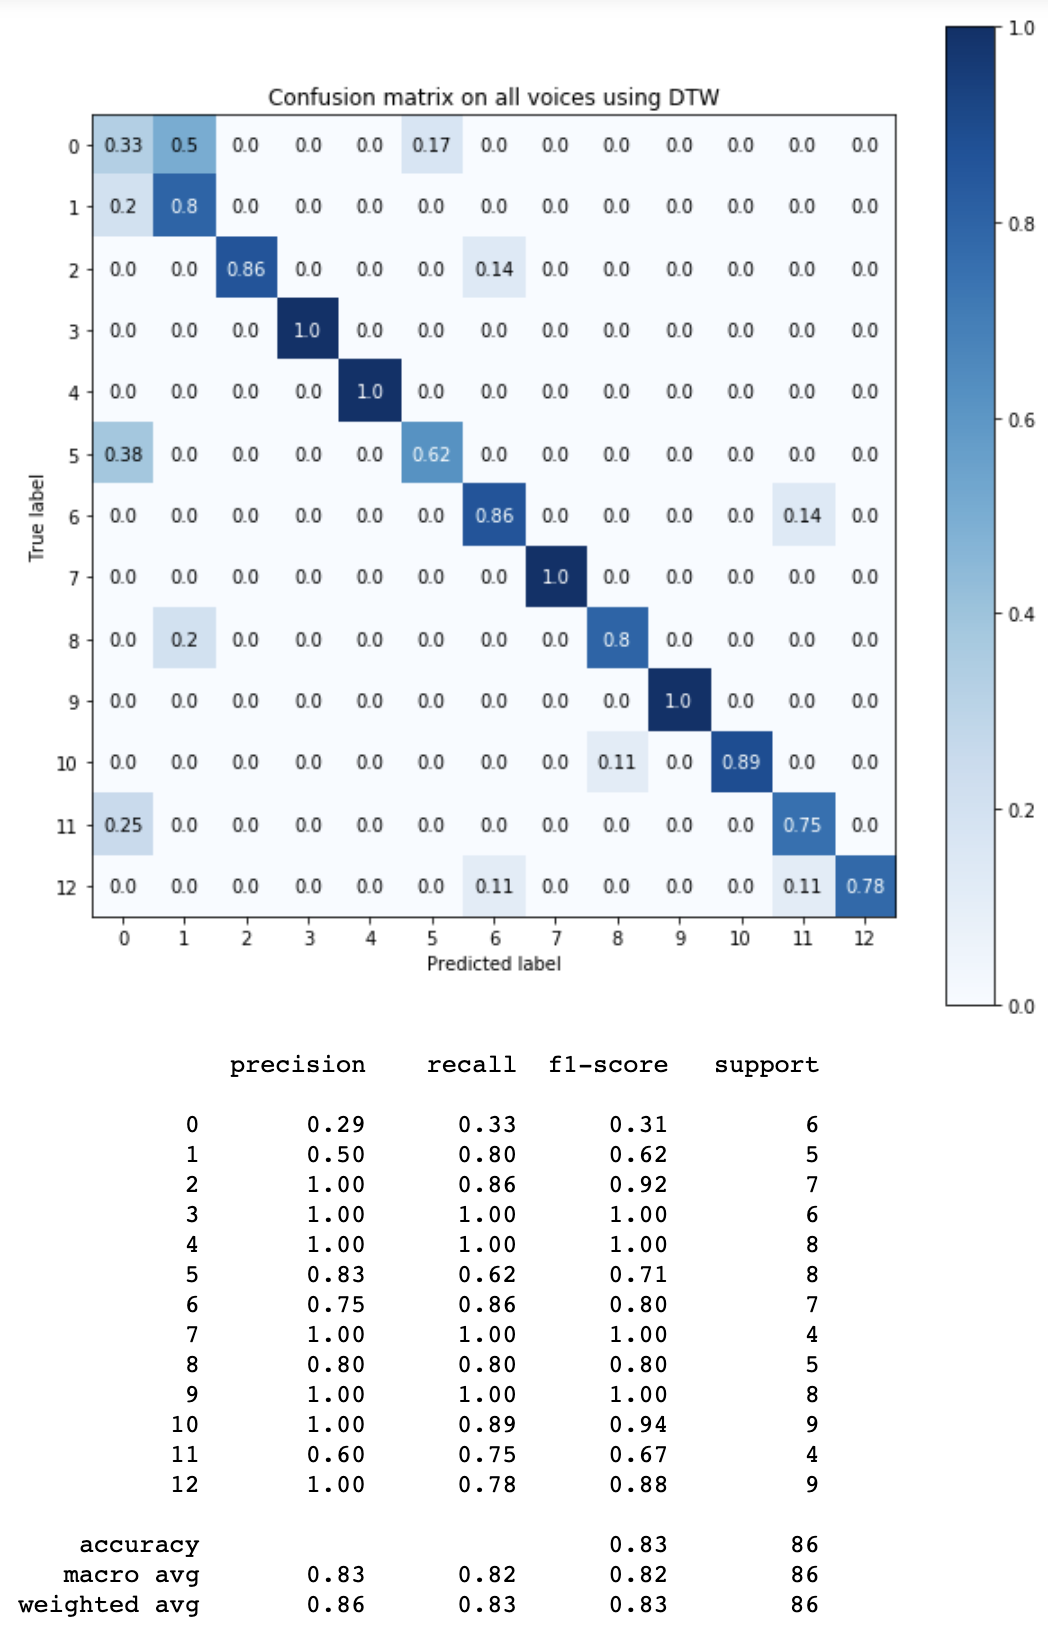
\includegraphics[width = \columnwidth]{./Figuras/dtwall}
  \caption{Evaluating DTW algorithm with normal (random noise and without noise) data}
  \label{fig:dtwall}
\end{figure}
\end{minipage}\qquad
\begin{minipage}[b]{.4\textwidth}
\begin{figure}[H]
  \centering
  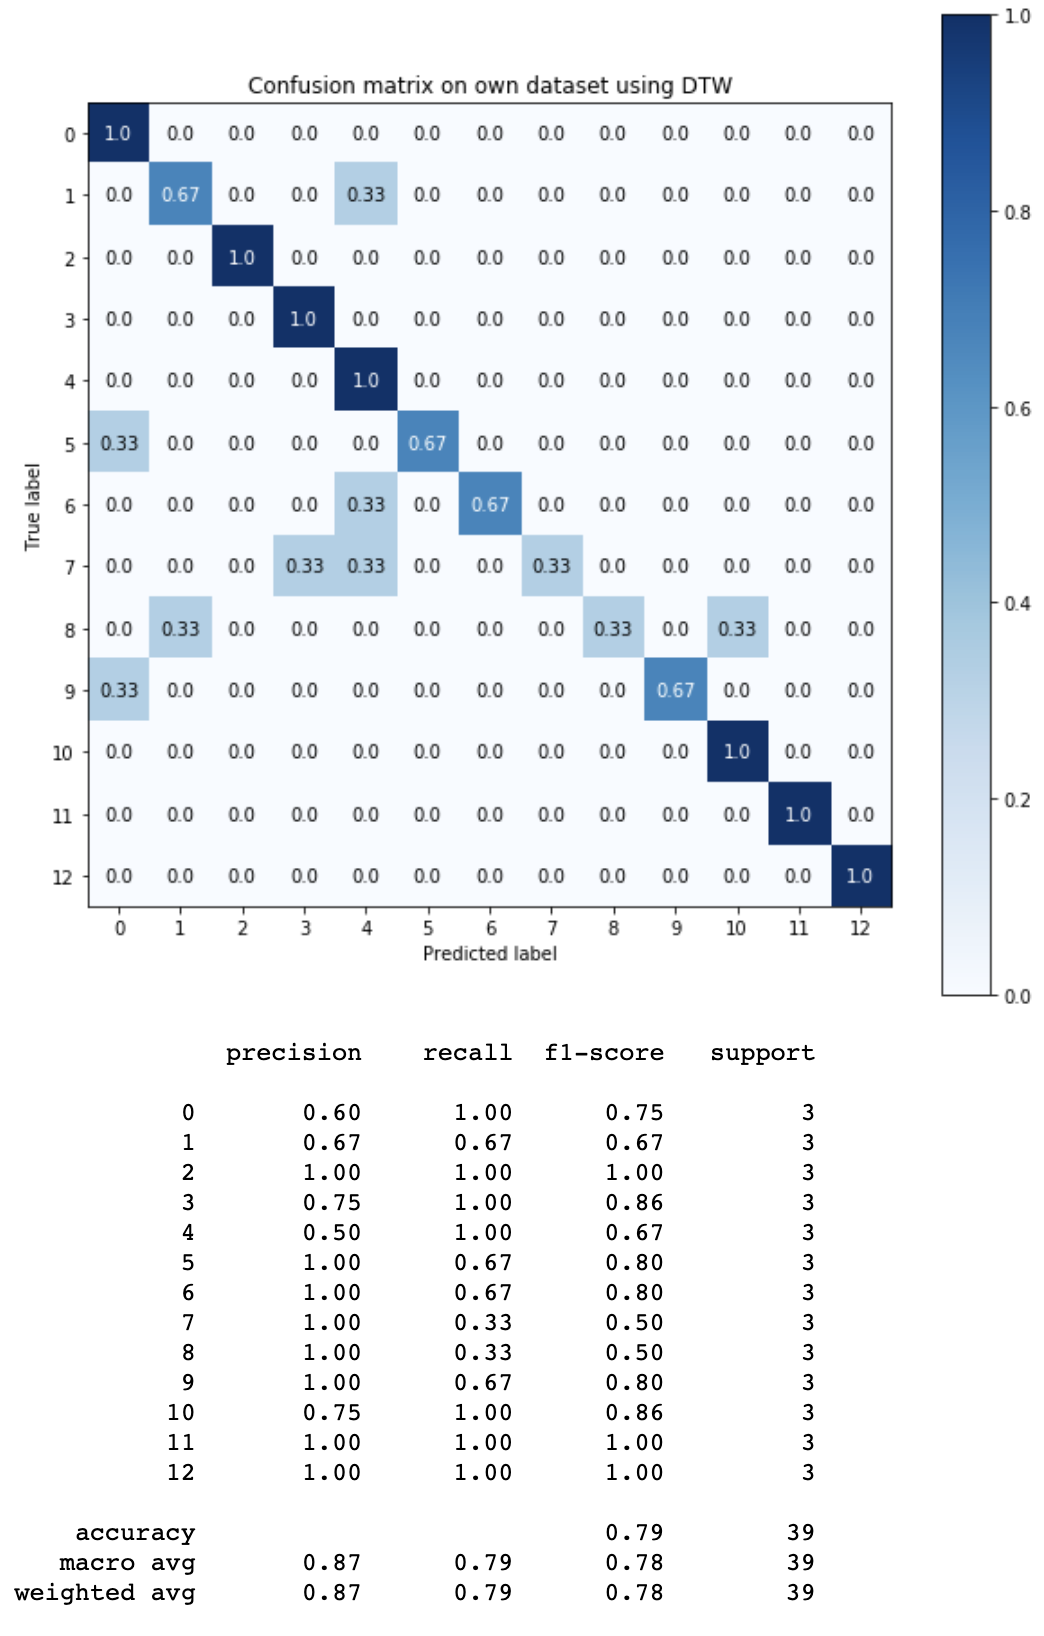
\includegraphics[width = \columnwidth]{./Figuras/dtwnewvoice}
   \caption{Evaluating DTW algorithm ability to new voice}
   \label{fig:dtwnewvoice}
\end{figure}
\end{minipage}
\end{figure*}
\subsection{PCA and KNN}
We have augmented dataset by changing pitch with Frequency (+15\%,+25\%,+50\%,-15\%,-25\%,-50\%). Which permits dataset is better make our model to do not depend on accent and reduce noise. In here, we implement following upgrade version: using delta and delta 2 of MFCC as Figure \ref{fig:pcs}\cite{8538414}.

\begin{figure}[H]
  \centering
  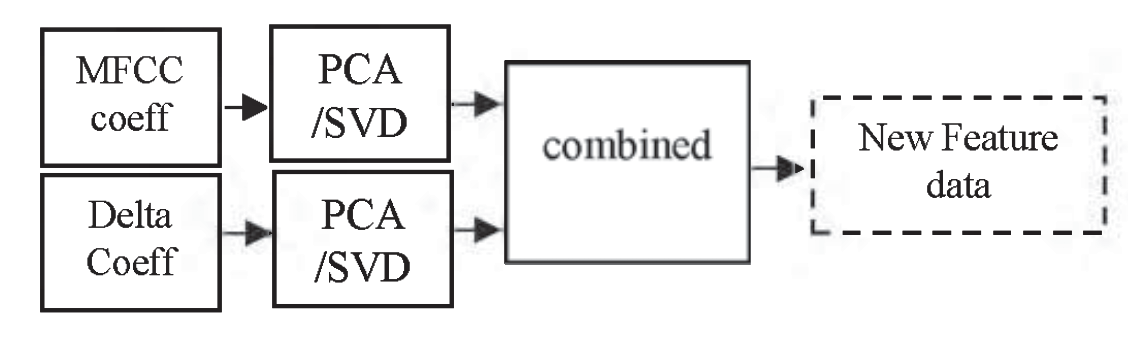
\includegraphics[width = 0.7\columnwidth]{./Figuras/pcs}
  \caption{The MFCC + Del + Del2 +PCA + KNN process.}
  \label{fig:pcs}
\end{figure}
And we have got best results on test data is 93\% as Figure \ref{fig:knnall} and 95\% on own data as Figure \ref{fig:knnown}.
\begin{figure*}
\centering
\begin{minipage}[b]{.4\textwidth}
\begin{figure}[H]
  \centering
  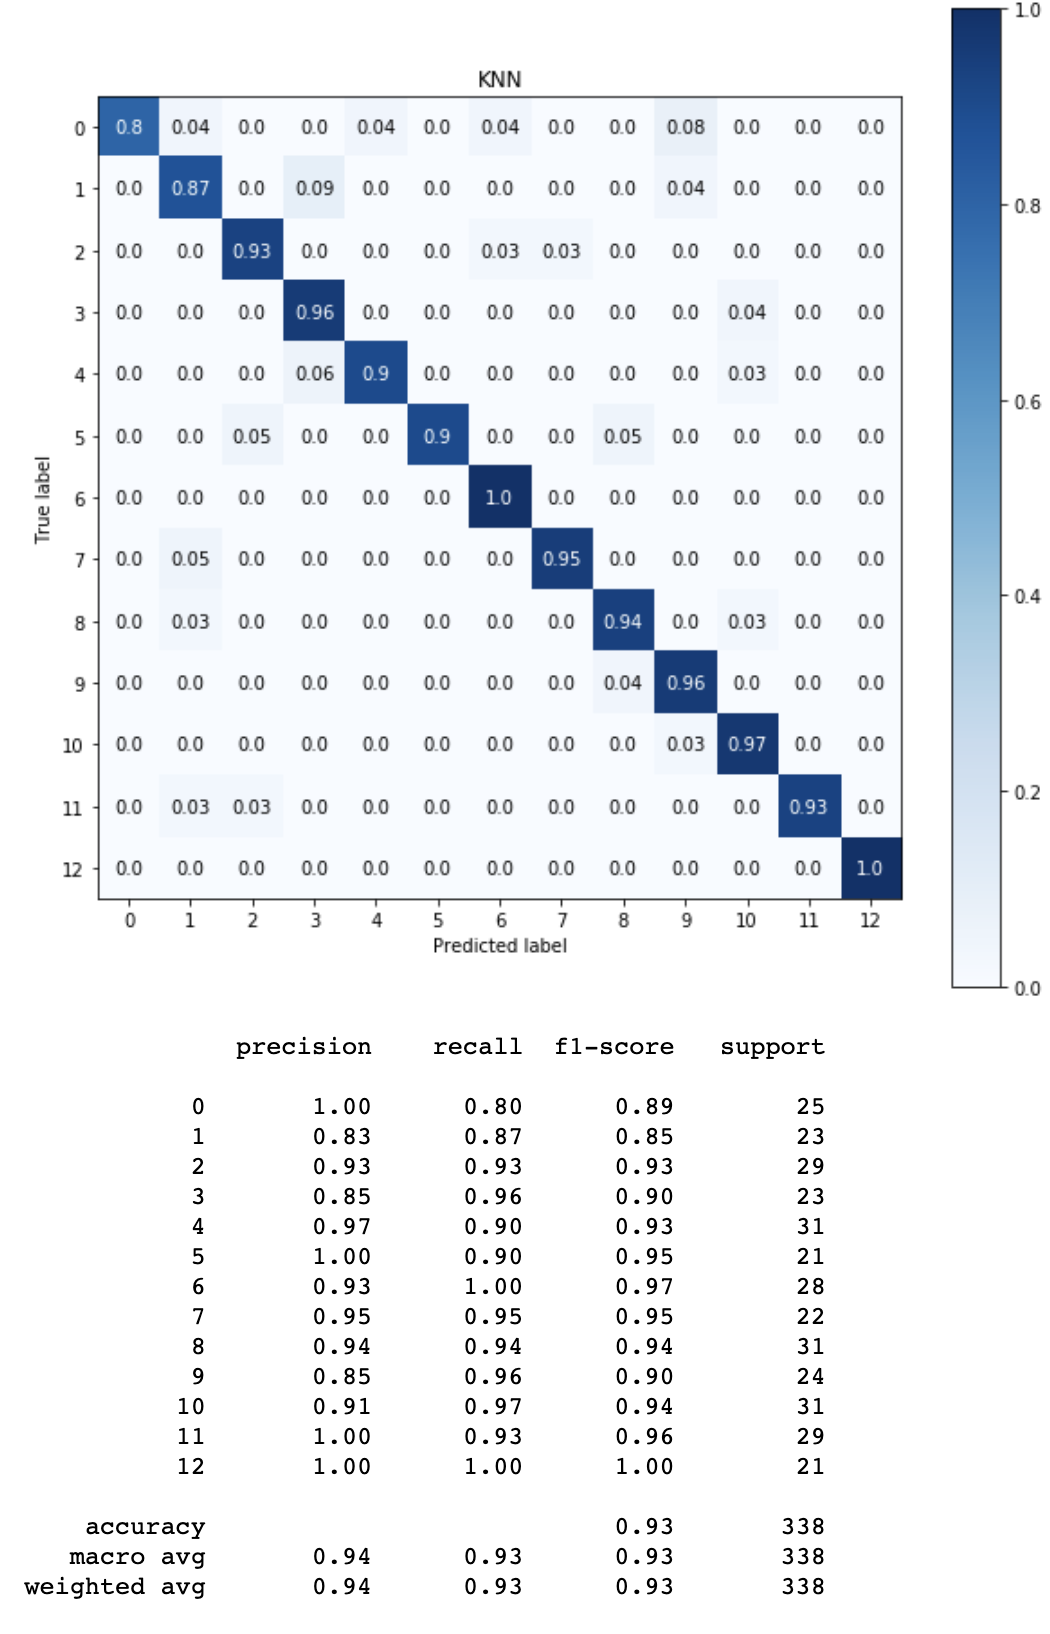
\includegraphics[width = \columnwidth]{./Figuras/knnall}
  \caption{Evaluating PCA+KNN model normal (random noise and without noise) data}
  \label{fig:knnall}
\end{figure}
\end{minipage}\qquad
\begin{minipage}[b]{.4\textwidth}
\begin{figure}[H]
  \centering
  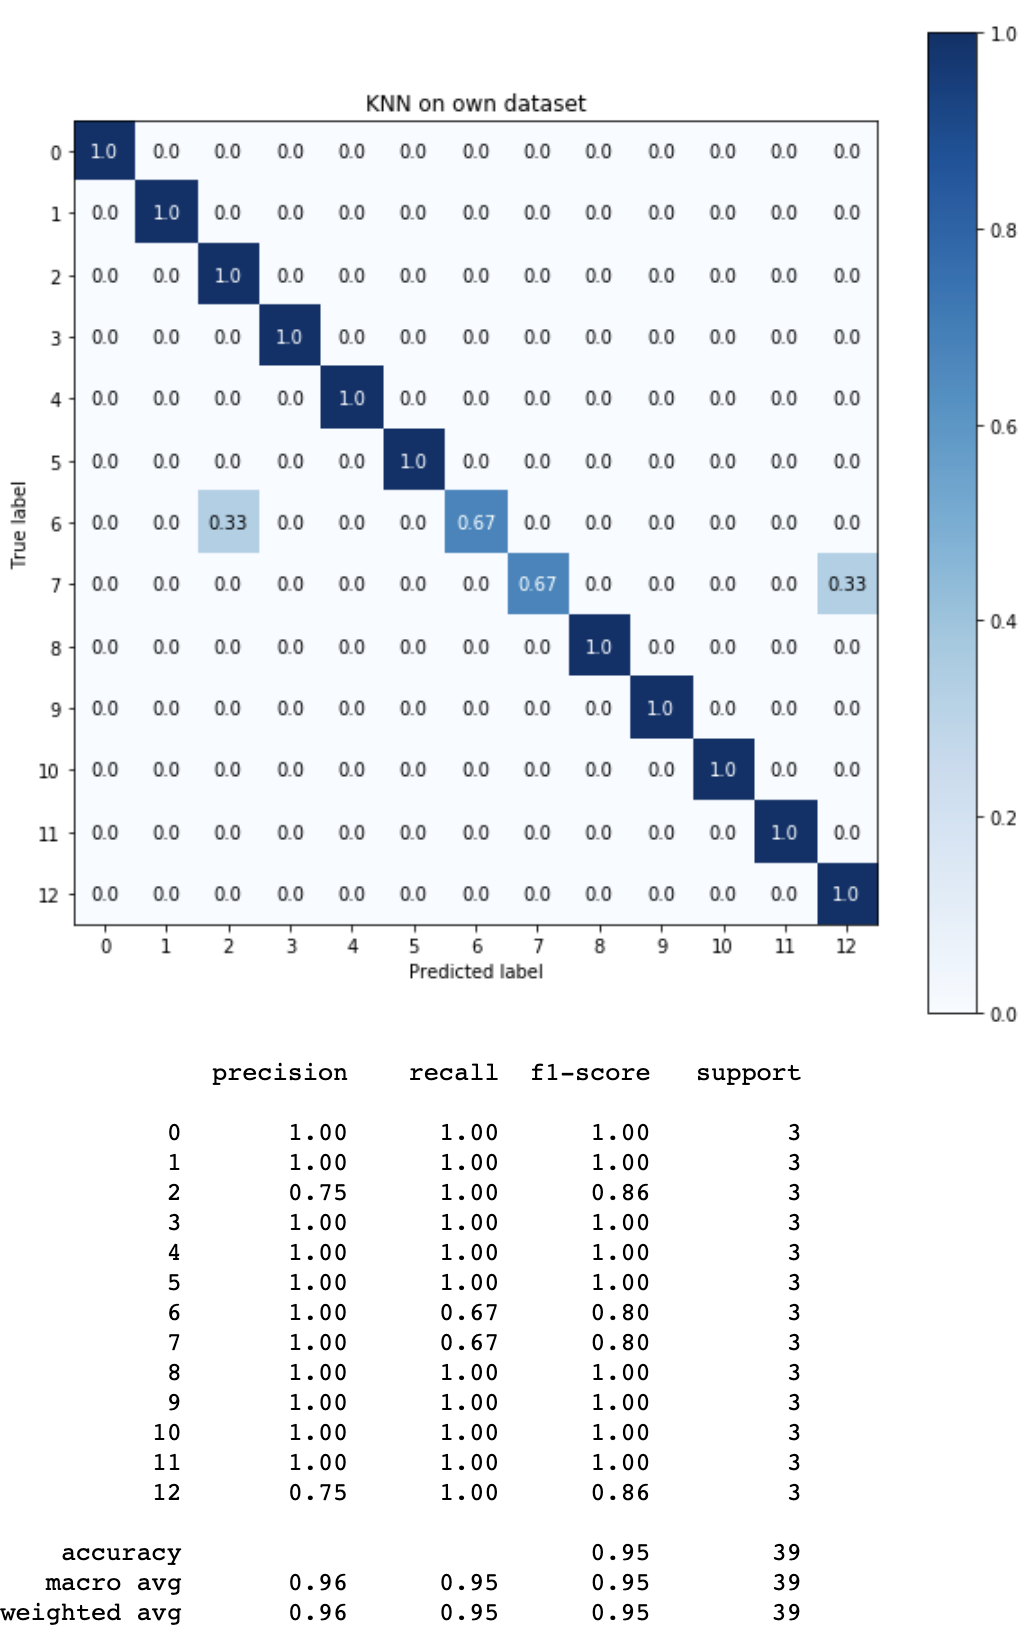
\includegraphics[width = \columnwidth]{./Figuras/knnown}
   \caption{Evaluating PCA+KNN ability to new voice}
   \label{fig:knnown}
\end{figure}
\end{minipage}
\end{figure*}

\subsection{CNN}
We have tried to train Deep Neural network model - CNN. Figure \ref{fig:cnnarch} present architecture CNN model with $14,301$ parameters. And Figure \ref{fig:losscnn} and \ref{fig:acccnn} show the loss and accuracy after 6000 epochs.
\begin{figure}[H]
  \centering
  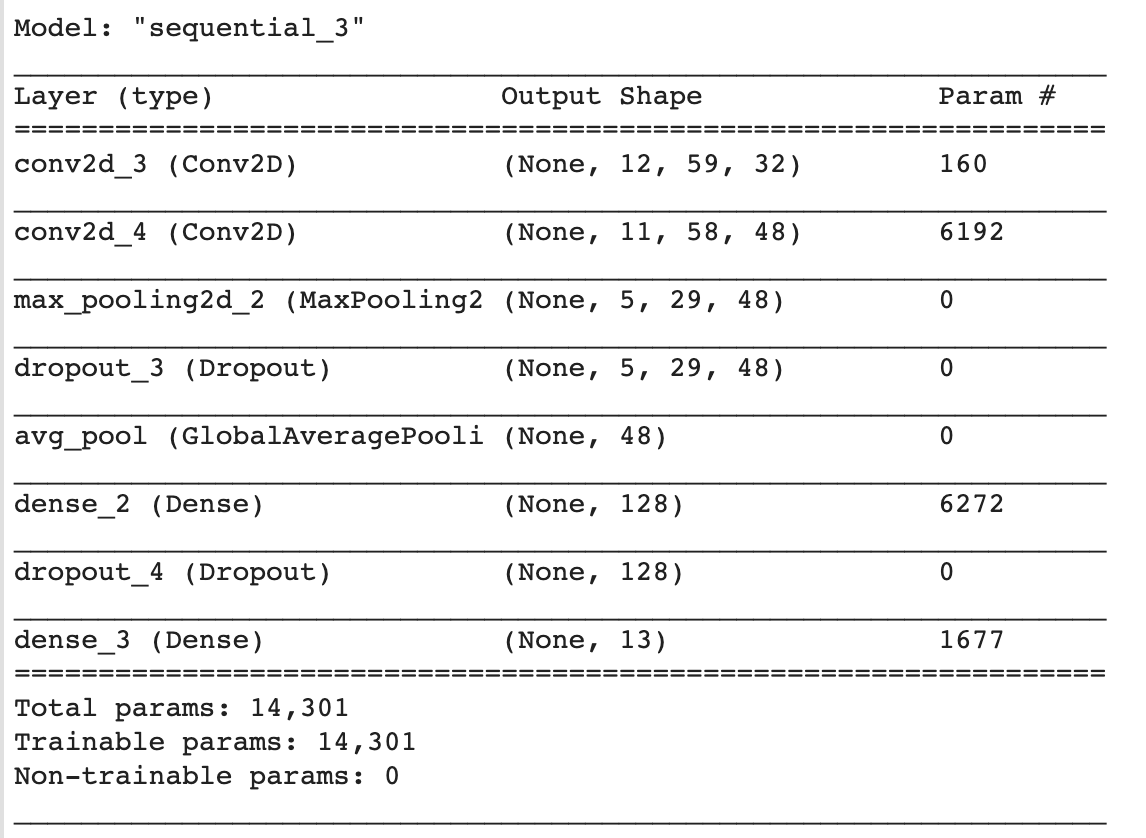
\includegraphics[width = 0.7\columnwidth]{./Figuras/cnnarch}
   \caption{The CNN architecture model}
   \label{fig:cnnarch}
\end{figure}

\begin{figure*}
\centering
\begin{minipage}[b]{.4\textwidth}
\begin{figure}[H]
  \centering
  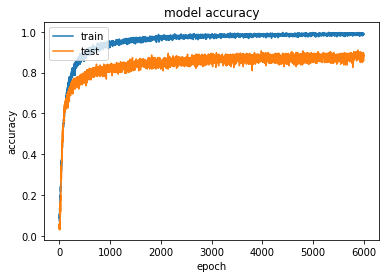
\includegraphics[width = \columnwidth]{./Figuras/losscnn}
  \caption{The loss and accuracy during training model.}
  \label{fig:losscnn}
\end{figure}
\end{minipage}\qquad
\begin{minipage}[b]{.4\textwidth}
\begin{figure}[H]
  \centering
  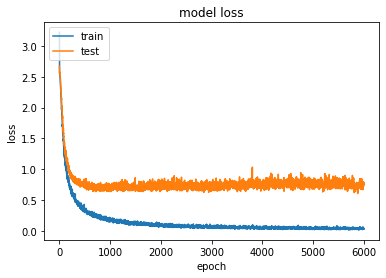
\includegraphics[width = \columnwidth]{./Figuras/acccnn}
   \caption{The loss and accuracy of test set.}
   \label{fig:acccnn}
\end{figure}
\end{minipage}
\end{figure*}

And we have got good results on test data is 91\% as Figure \ref{fig:cnnall} and 79\% on own data as Figure \ref{fig:cnnown}.

\begin{figure*}
\centering
\begin{minipage}[b]{.4\textwidth}
\begin{figure}[H]
  \centering
  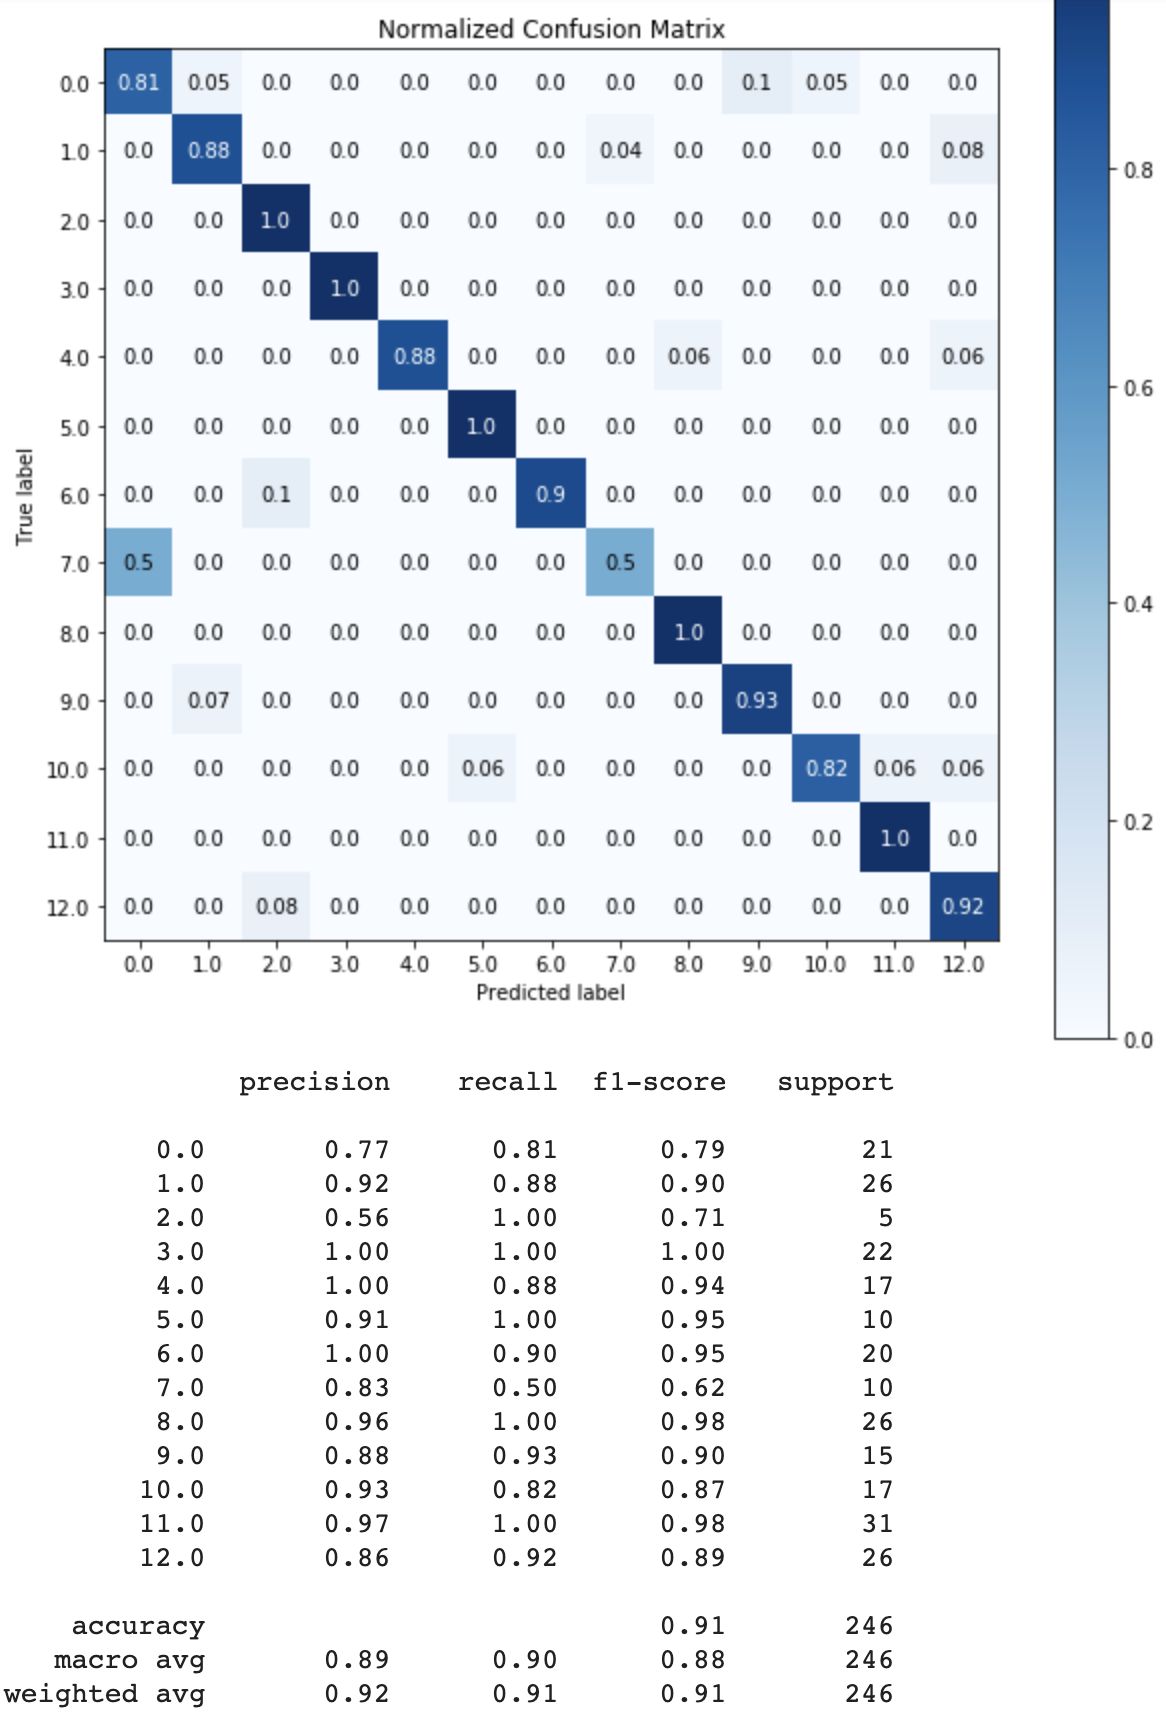
\includegraphics[width = \columnwidth]{./Figuras/cnnall}
  \caption{Evaluating CNN model normal (random noise and without noise) data}
  \label{fig:cnnall}
\end{figure}
\end{minipage}\qquad
\begin{minipage}[b]{.4\textwidth}
\begin{figure}[H]
  \centering
  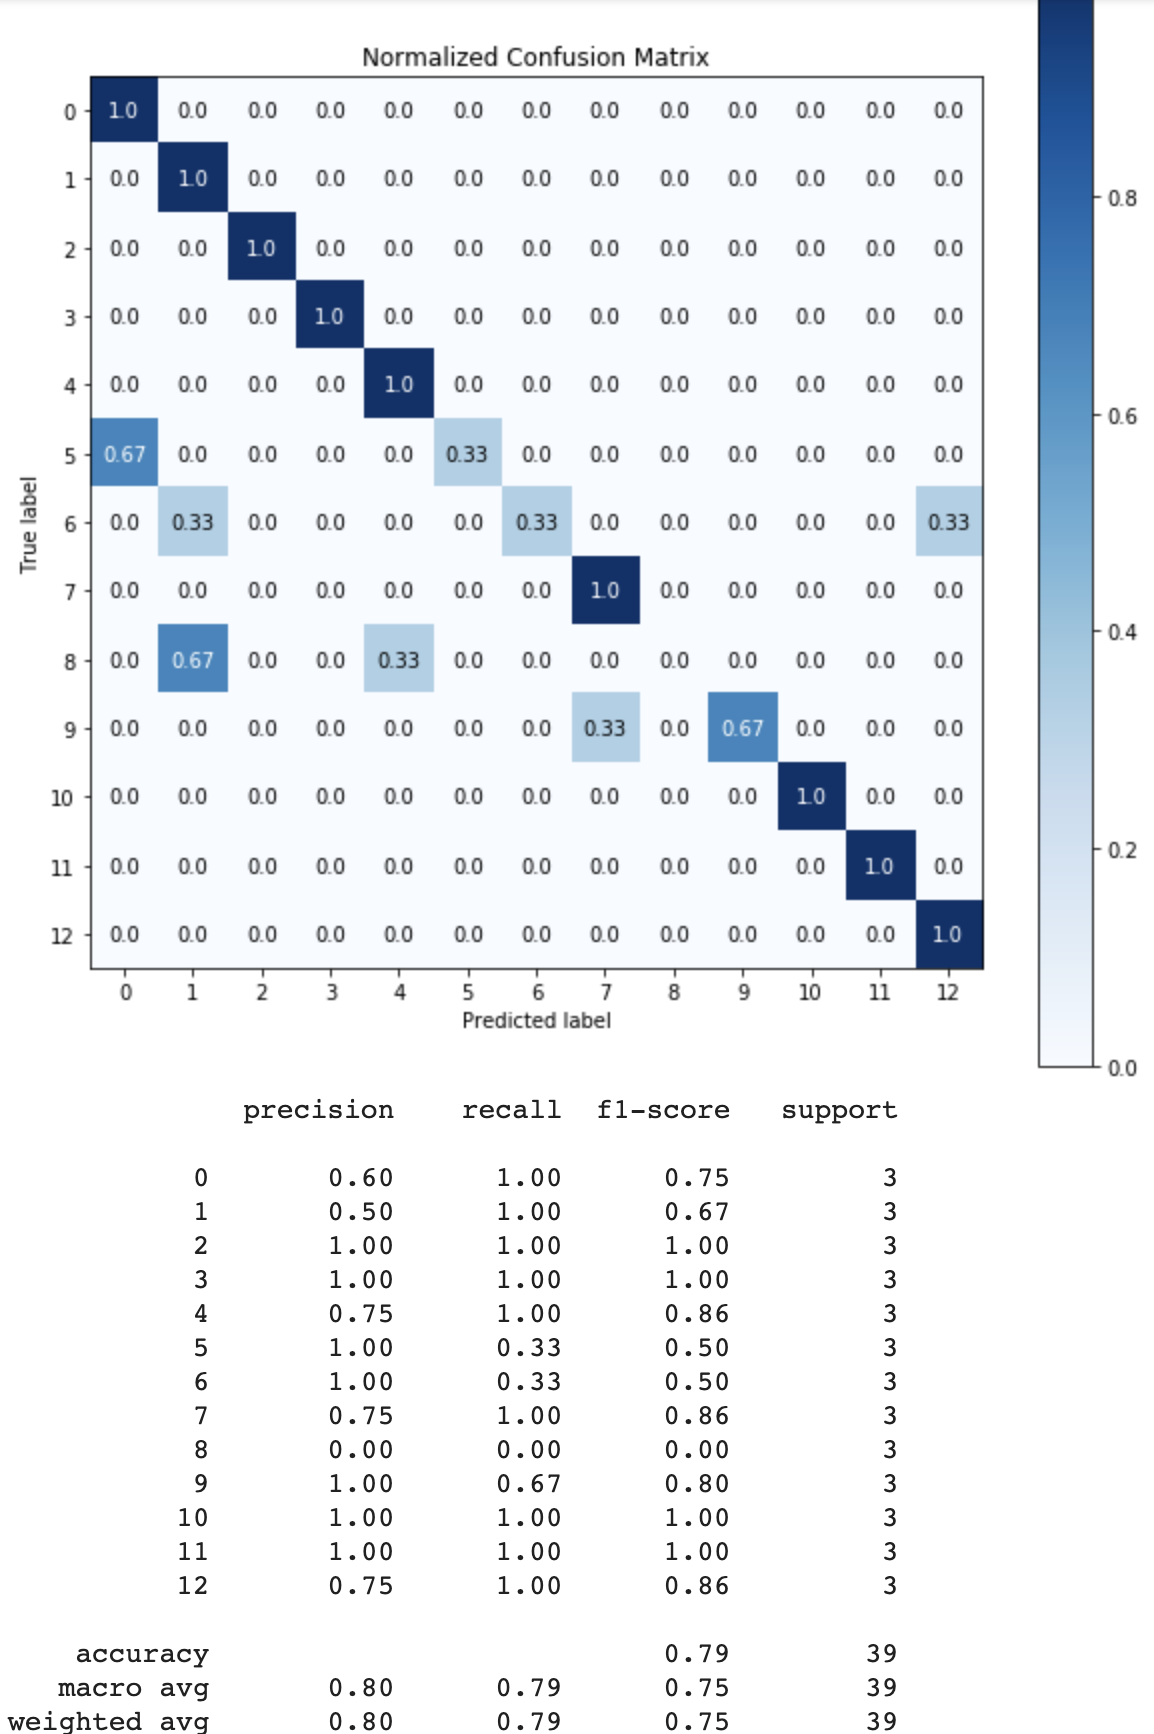
\includegraphics[width = \columnwidth]{./Figuras/cnnown}
   \caption{Evaluating CNN ability to new voice}
   \label{fig:cnnown}
\end{figure}
\end{minipage}
\end{figure*}

\section{conclusions}
The primary objective, we have successfully implemented DTW algorithm, PCA, KNN and CNN methods and get good results. We see that, data augmentation make better accuracy and combining MFCC + del + del2 and PCA + KNN has best results. Although, using DTW on data augmentation is more expensive, I think it's a simple method and good result.

\printbibliography%% Referências

%% Fim do documento
\end{document}
